\section{Loi de conservation de la charge}

    \subsection{Géométrie 1D}

        On considère la Figure~\ref{fig:conservation_charge_1d}.

        \begin{figure}
            \centering
            \tikzsetnextfilename{conservation_charge_1d}
            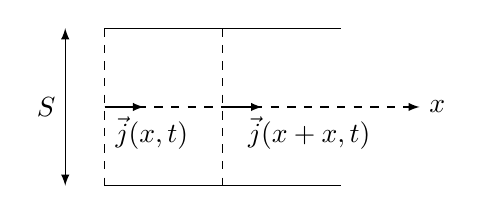
\begin{tikzpicture}[scale=1]  
                % \helpgrid{3}{3}
                \draw[dashed,-latex] (0,0)--++(4,0) node [right] {$x$};
                \draw (0,-1)--++(3,0);
                \draw (0,1)--++(3,0);
                \draw[-latex] (0,0)--++(0.5,0) node [below,pos=1.2] {$\vec{j}(x,t)$};
                \draw[-latex] (1.5,0)--++(0.5,0) node [below, pos=2.2] {$\vec{j}(x+\rmd x,t)$};
                \draw[dashed] (0,1)--++(0,-2);
                \draw[dashed] (1.5,1)--++(0,-2);
                \draw[latex-latex] (-0.5,1)--++(0,-2) node [left,midway] {$S$};
            \end{tikzpicture}
            \caption{Loi de conservation de la charge 1D.}    
            \label{fig:conservation_charge_1d}
        \end{figure}

        La charge entrant algébriquement dans $S\rmd x$ pendant $\rmd t$ est 
        \begin{align*}
            \delta Q_e
            &=
            j(x,t)S\rmd t-j(x+\rmd x,t)S\rmd t,\\
            &=
            S\rmd t\left[
                j(x,t)-j(x+\rmd x,t)
            \right],\\
            &=-S\rmd t\rmd x\frac{\partial j}{\partial x}(x,t).
        \end{align*}

        La variation $\rmd Q$ de la charge dans la tranche $S\rmd x$ est 
        \begin{align*}
            \rmd Q
            &=
            \rho(x,t+\rmd t)S\rmd x-\rho(x,t)S\rmd x,\\
            &=
            S\rmd x\left(\rho(x,t+\rmd t)-\rho(x,t)\right),\\
            &=
            \frac{\partial\rho}{\partial t}(x,t)S\rmd x\rmd t.
        \end{align*}

        \paragraph{Postulat : conservation de la charge.}

            On doit avoir 
            \begin{equation*}
                \boxed{
                    \rmd Q=\delta Q_e.
                }
            \end{equation*}

            Alors l'équation locale de la conservation de la charge s'écrit
            \begin{equation*}
                \boxed{
                    \frac{\partial\rho}{\partial t}(x,t)+\frac{\partial j}{\partial x}(x,t)=0.
                }
            \end{equation*}

    \subsection{Équation intégrale de conservation de la charge}

        Dans le cas général, on se reporte à la Figure~\ref{fig:equation*_integrale_conservation_charge}.

        \begin{figure}
            \centering
            \tikzsetnextfilename{equation*_integrale_conservation_charge}
            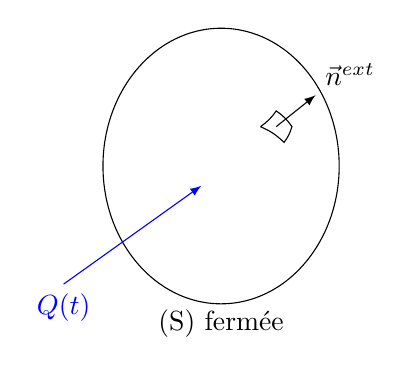
\begin{tikzpicture}[scale=1]  
                \draw (0,0) ellipse (1.5 and 1.75);
                \node at (0,-2) {(S) fermée};
                \draw[latex-,draw=blue,text=blue] (-0.25,-0.25)--(-2,-1.5) node [below]{$Q(t)$};
                \draw (0.5,0.5) to[bend right=10] (0.7,0.7) to[bend left=10] (0.9,0.5) to[bend left=10] (0.8,0.3) to[bend right=10] (0.5,0.5);
                \draw[-latex] (0.7,0.5)--++(0.5,0.4) node [above right] {$\vec{n}^{\text{ext}}$};
            \end{tikzpicture}
            \caption{Équation intégrale de conservation de la charge.}    
            \label{fig:equation*_integrale_conservation_charge}
        \end{figure}

        Le flux sortant de $\vec{j}$ est 
        \begin{equation*}
            i_S^{\text{ext}}=\oiint_{S}\vec{j}\cdot\vec{n}^{\text{ext}}\rmd S.
        \end{equation*}

        La conservation de la charge s'écrit alors
        \begin{equation*}
            \boxed{
                \frac{\rmd Q}{\rmd t}=-i_{S}^{\text{ext}}(t)=-\oiint_{S}\vec{j}\cdot\vec{n}^{\text{ext}}\rmd S.
            }
        \end{equation*}

    \subsection{Flux et opérateur \og divergence\fg}

        Dans le cas unidimensionnel de la Figure~\ref{fig:conservation_charge_1d}, en notant ($\Sigma$) la surface fermée comprise entre $x$ et $x+\rmd x$ et les bords en haut et en bas, on a 
        \begin{align*}
            i_{\Sigma}^{\text{ext}}(t)
            &=
            \oiint_{\Sigma}\vec{j}\cdot\vec{n}^{\text{ext}}\rmd\Sigma,\\
            &=
            \iint_{\text{bords}}\vec{j}\cdot\vec{n}_{\text{bords}}\rmd\Sigma+(-\vec{j}(x,t)\times S)+(j(x+\rmd x,t)\times S),\\
            &= 0 +\frac{\partial j}{\partial x}(x,t)\times S\rmd x,\\
            &=\frac{\partial j}{\partial x}(x,t) \times V.
        \end{align*}

        Ainsi, le flux est proportionnel au volume.

        Dans le cas à trois dimensions, on se reporte à la Figure~\ref{fig:flux_operateur_divergence_trois_dimensions}. On se donne un champ $\vec{A}(x,y,z,t)$, et on suppose le cube assez petit pour qu'il soit uniforme sur chaque face. On numérote les faces (1: gauche, 2: droite, 3: bas, 4:haut, 5: derrière, 6: devant).

        \begin{figure}
            \centering
            \tikzsetnextfilename{flux_operateur_divergence_trois_dimensions}
            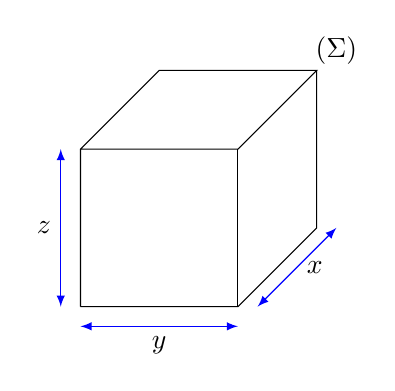
\begin{tikzpicture}[scale=1]  
                \draw (0,0)--(0,2)--(1,3)--(3,3)--(2,2)--(0,2);
                \draw (0,0)--(2,0)--(3,1)--(3,3);
                \draw (2,0)--(2,2);
                \draw [latex-latex, draw=blue] (-0.25,0)--++(0,2) node [left,midway] {$\rmd z$};
                \draw [latex-latex, draw=blue] (0,-0.25)--++(2,0) node [below,midway] {$\rmd y$};
                \draw [latex-latex, draw=blue] (2.25,0)--++(1,1) node [right,midway] {$\rmd x$};
                \node at (3.25,3.25) {$(\Sigma)$};
            \end{tikzpicture}
            \caption{Flux de courant sortant en trois dimensions.}    
            \label{fig:flux_operateur_divergence_trois_dimensions}
        \end{figure}

        On cherche la quantité $\delta \phi^{\text{ext}}$ sortant du cube à cause du flux de $\vec{A}$ via la surface de $(\Sigma)$.
        On définit donc 
        \begin{equation*}
            \delta \phi^{\text{ext}}\coloneqq\oiint_{(\Sigma)}\vec{A}\cdot\vec{n}^{\text{ext}}\rmd\Sigma.
        \end{equation*}
        On a alors
        \begin{enumerate}[label=(\arabic*)]
            \item $\vec{n}^{\text{ext}}=-\vec{u_y}$ : $\delta \phi_{1}^{\text{ext}}=-A_y(x,y,z,t)\times(\rmd x\rmd z)$;
            \item $\vec{n}^{\text{ext}}=\vec{u_y}$ : $\delta \phi_{2}^{\text{ext}}=+A_y(x,y,z,t)\times(\rmd x\rmd z)$;
            \item $\vec{n}^{\text{ext}}=-\vec{u_z}$ : $\delta \phi_{3}^{\text{ext}}=-A_z(x,y,z,t)\times(\rmd x\rmd y)$;
            \item $\vec{n}^{\text{ext}}=\vec{u_z}$ : $\delta \phi_{4}^{\text{ext}}=+A_z(x,y,z,t)\times(\rmd x\rmd y)$;
            \item $\vec{n}^{\text{ext}}=-\vec{u_x}$ : $\delta \phi_{5}^{\text{ext}}=-A_x(x,y,z,t)\times(\rmd y\rmd z)$;
            \item $\vec{n}^{\text{ext}}=-\vec{u_x}$ : $\delta \phi_{6}^{\text{ext}}=+A_x(x,y,z,t)\times(\rmd y\rmd z)$.
        \end{enumerate}

        On fait la somme algébrique
        \begin{equation*}
            \begin{aligned}
                1+2 &: \frac{\partial A_y}{\partial y}(x,y,z,t)\times\rmd y\rmd x\rmd z,\\
                3+4 &: \frac{\partial A_z}{\partial z}(x,y,z,t)\times\rmd z\rmd x\rmd y,\\
                5+6 &: \frac{\partial A_x}{\partial x}(x,y,z,t)\times\rmd x\rmd y\rmd z.
            \end{aligned}
        \end{equation*}

        Ainsi,
        \begin{equation*}
            \boxed{
                \delta \phi^{\text{ext}}=\left[
                    \frac{\partial A_x}{\partial x}+\frac{\partial A_y}{\partial y}+\frac{\partial A_z}{\partial z}
                \right]\times \rmd V=(\div\vec{A})\rmd V.
            }
        \end{equation*}

        \paragraph{Théorème-définition d'Ostrogradski.}

            Soit $\vec{A}(\vec{r},t)=\vec{A}(x,y,z,t)$ un champ de vecteurs de classe $\mathcal{C}^{1}$. Alors on a 
            \begin{equation*}
                \boxed{
                    \oiint_{S}\vec{A}\cdot\vec{n}^{\text{ext}}\rmd S=\iiint_{V}\div\vec{A}\rmd V.
                }
            \end{equation*}

            En coordonnées cartésiennes, la divergence de $\vec{A}$ s'écrit 
            \begin{equation*}
                \boxed{
                    \div\vec{A}=\frac{\partial A_x}{\partial x}+\frac{\partial A_y}{\partial y}+\frac{\partial A_z}{\partial z}.
                }
            \end{equation*}

            L'opérateur symbolique (réservé aux coordonnées cartésiennes) est \og nabla\fg, qui s'écrit
            \begin{equation*}
                \boxed{
                    \vecnabla=\begin{pmatrix}
                        \frac{\partial}{\partial x}\\[0.2cm]
                        \frac{\partial}{\partial y}\\[0.2cm]
                        \frac{\partial}{\partial z}
                    \end{pmatrix}.
                }
            \end{equation*}

            On a alors $\div\vec{A}=\vecnabla\cdot\vec{A}$.

    \subsection{Équation locale de conservation de la charge en trois dimensions.}

        Pour une géométrie quelconque, la variation de $Q(t)$ contenue dans un volume $V$ est 
        \begin{equation*}
            \rmd Q=\iiint_{V}\left[\rho(\vec{r},t)-\rho(\vec{r},t+\rmd t)\right]\rmd V,
        \end{equation*}
        d'où 
        \begin{equation*}
            \boxed{
                \rmd Q=\left(\iiint_{V}\frac{\partial \rho}{\partial t}(\vec{r},t)\rmd V\right)\rmd t.
            }
        \end{equation*}

        La charge algébrique $\delta Q_{S}^{\text{ext}}$ traversant une surface $S$ orientée vers l'extérieur pendant $\rmd t$ est 
        \begin{equation*}
            \delta Q_S^{\text{ext}}=i_{S}^{\text{ext}}(t)\times\rmd t=\left[
                \oiint_{S}\vec{j}\cdot\vec{n}^{\text{ext}}\rmd S
            \right]\rmd t.
        \end{equation*}
        Or on a 
        \begin{equation*}
            \oiint_{S}\vec{j}\cdot\vec{n}^{\text{ext}}\rmd S=\iiint_{V}\div\vec{j}\cdot\rmd V,
        \end{equation*}
        donc
        \begin{equation*}
            \boxed{
                \delta Q_S^{\text{ext}}=\left(
                    \iiint_{V}(\div\vec{j}\rmd V)
                \right)\rmd t.
            }
        \end{equation*}

        La conservation de la charge s'écrit alors $\rmd Q=-\delta Q_S^{\text{ext}}$, qui est une équation globale :
        \begin{equation*}
            \iiint\left(\frac{\partial\rho}{\partial t}+\div\vec{j}\right)\rmd V=0.
        \end{equation*}
        Ceci ayant lieu pour tout volume $V$ de taille au moins mésoscopique, on a l'équation locale de la conservation de la charge :
        \begin{equation*}
            \boxed{
                \frac{\partial\rho}{\partial t}+\div\vec{j}=0.
            }
        \end{equation*}

    \subsection{Cas du régime stationnaire/permanent}

        Dans de cas, on a 
        \begin{equation*}
            \boxed{
                \dfrac{\partial\rho}{\partial t}=0,\qquad\div\vec{j}=0.
            }
        \end{equation*}

        En conséquence, 
        \begin{enumerate}[label=(\roman*)]
            \item $\vec{j}$ est à flux conservatif. En effet,
            \begin{equation*}
                i_S^{\text{ext}}=\oiint_{S}\vec{j}\cdot\vec{n}^{\text{ext}}\rmd S=\iiint_{V}\div\vec{j}\rmd V=0.
            \end{equation*}
            \item $i=$constante le long d'un tube de courant (régime permanent). Un tube de courant est un ensemble de lignes de courant s'appuyant sur un contour fermé. Ces lignes de courant sont des courbes tangentes à $\vec{j}$ en tout point.
            \item Loi des n\oe uds : en un n\oe ud où différents courants arrivent, on a 
            \begin{equation*}
                \boxed{
                    \sum_{k}\varepsilon_{k}i_k=0,
                }
            \end{equation*}
            avec $\varepsilon_{k}=\pm1$.
        \end{enumerate}